\documentclass{article}
\usepackage{tikz}
\usetikzlibrary{arrows.meta,positioning,calc,shapes.geometric}
\pagestyle{empty}
\begin{document}
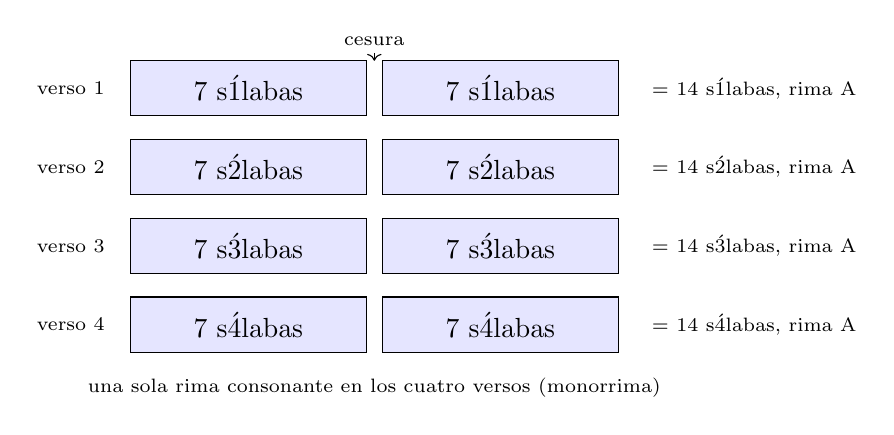
\begin{tikzpicture}

\foreach \i/\y in {1/3.0,2/2.0,3/1.0,4/0.0} {
  \node[font=\scriptsize, anchor=east] at (-0.2,\y) {verso \i};
  \node[draw, fill=blue!10, minimum width=3.0cm, minimum height=0.7cm] at (1.5,\y) {7 sílabas};
  \node[draw, fill=blue!10, minimum width=3.0cm, minimum height=0.7cm] at (4.7,\y) {7 sílabas};
  \node[font=\scriptsize, anchor=west] at (6.5,\y) {= 14 sílabas, rima A};
}
\node[font=\scriptsize] at (3.1,3.6) {cesura};
\draw[->] (3.1,3.45) -- (3.1,3.35);
\node[font=\scriptsize] at (3.1,-0.8) {una sola rima consonante en los cuatro versos (monorrima)};

\end{tikzpicture}
\end{document}
